\documentclass{article}

%**************************************************************
% Importazione package
%**************************************************************

% permette di modificare i margini
%\usepackage[top=3.1cm, bottom=3.1cm, left=2.2cm, right=2.2cm]{geometry}
\usepackage[a4paper]{geometry}

% necessario per risolvere il problema del carattere invisibile per l'a capo
% \DeclareUnicodeCharacter{00A0}{ }

% per scrivere in italiano e in inglese;
% l'ultima lingua (l'italiano) risulta predefinita
\usepackage[english, italian]{babel}

% imposta lo stile italiano per i paragrafi
\usepackage{parskip}

% fornice elenchi numerati in ordine inverso
\usepackage{etaremune}

% comandi per l'appendice
\usepackage{appendix}
\renewcommand\appendixtocname{Appendici}
\renewcommand{\appendixpagename}{Appendici}

% numera anche i paragrafi
\setcounter{secnumdepth}{6}

% elenca anche i paragrafi nell'indice
\setcounter{tocdepth}{6}

% permetti di definire dei colori
\usepackage[usenames,dvipsnames]{color}

% permette di inserire le immagini/tabelle esattamente dove viene usato il
% comando \begin{figure}[H] ... \end{figure}
% evitando che venga spostato in automatico
\usepackage{float}

% permette l'inserimento di url e di altri tipi di collegamento
\usepackage[colorlinks=true]{hyperref}

\hypersetup{
    colorlinks=true, % false: boxed links; true: colored links
    citecolor=black,
    filecolor=black,
    linkcolor=black, % color of internal links
    urlcolor=Maroon  % color of external links
}

% immagini
\usepackage{graphicx}

% permette di riferirsi all'ultima pagina con \pageref{LastPage}
\usepackage{lastpage}

% tabelle su più pagine
\usepackage{longtable}

% per avere dei comandi in più da poter usare sulle tabelle
\usepackage{booktabs}

% tabelle con il campo X per riempire lo spazio rimanente sulla riga
\usepackage{tabularx}

% multirow per tabelle
\usepackage{multirow}

% colore di sfondo per le celle
\usepackage[table]{xcolor}
%\rowcolors{2}{gray!25}{} % Colora righe alterne in grigio (non funziona bene)

% permette di fare longtable larghe tutta la pagina (parametro x)
% su Ubuntu non si può installare il pacchetto, deve essere in model/
\usepackage{tabu}

% imposta lo spazio tra le righe di una tabella
\setlength{\tabulinesep}{6pt}

% definisci un nuovo tipo di colonna P che permette di andare a capo con \newline
% e giustificata a sinistra
\usepackage{array}
\usepackage{ragged2e}
\newcolumntype{P}[1]{>{\RaggedRight \hspace{0pt}}m{#1}}

% personalizza l'intestazione e piè di pagina
\usepackage{fancyhdr}

% permette di inserire caratteri speciali
\usepackage{textcomp}

% permette di aggiustare i margini e centrare tabelle e figure
\usepackage{changepage}

%Permette di includere i grafici a barre
%IMPORTANTE: deve essere caricato prima di /pgfgantt altrimenti causa conflitto
\usepackage{pgfplots}

% permette di includere i diagrammi Gantt
% su Ubuntu non si può installare il pacchetto, deve essere in model/
\usepackage{pgfgantt}

% permette di includere i grafici a torta
\usepackage{pgf-pie}

% necessario per pgf-pie
\usepackage{tikz}

% permette i path delle immagini con gli spazi
\usepackage{grffile}

% ruota le immagini
\usepackage{rotating}

% permetti di calcolare le larghezze facendo calcoli
\usepackage{calc}


%%
%% Definizione di path globali
%%
% Path assoluta a questa directory, va passato come argomento il resto della path
\newcommand{\ModelPath}[1]{/data/sources/model/#1}

% Path per accedere a modelassets
\newcommand{\ModelAssets}[1]{\ModelPath{modelassets}/#1}

% Path globali per la ricerca di immagini
\graphicspath{
	{/data/logo/PNG}
	{/data/logo/Square}
}



\fancypagestyle{plain}{
	% cancella tutti i campi di intestazione e piè di pagina
	\fancyhf{}
	\lhead{
		
\includegraphics[width=1.5cm, keepaspectratio=true]{argo_icona.png}
		\parbox[b]{5cm}{
			\emph{\GroupName{}} \vspace{0pt} \\
			\emph{Progetto \ProjectName{}} \vspace{0pt}
		}
	}
	\chead{}


	\lfoot{
		\DocTitle{} \\
		% differenzia a seconda che \DocVersion{} stampi testo o no
		\setbox0=\hbox{\DocVersion{}\unskip}\ifdim\wd0=0pt
			% nulla
		\else
			v \DocVersion{}
		\fi
	}
	\rfoot{\thepage{} di \pageref{LastPage}}

	% Visualizza una linea orizzontale in cima e in fondo alla pagina
	\renewcommand{\headrulewidth}{0.3pt}
	\renewcommand{\footrulewidth}{0.3pt}
}
\setlength{\headheight}{30pt}
\pagestyle{plain}

% allarga l'header a tutta la pagina
%\fancyhfoffset[L]{\oddsidemargin + \hoffset + 1in}
%\fancyhfoffset[R]{\evensidemargin + \marginparwidth - \marginparsep}

% Per inserire del codice sorgente formattato
\usepackage{listings}
\definecolor{darkgray}{rgb}{.4,.4,.4}
\definecolor{purple}{rgb}{0.65, 0.12, 0.82}
\definecolor{mygreen}{rgb}{0,0.6,0}
\definecolor{mygray}{rgb}{0.5,0.5,0.5}
\definecolor{mymauve}{rgb}{0.58,0,0.82}

\lstset{
  extendedchars=true,          % lets you use non-ASCII characters
  inputencoding=utf8,   % converte i caratteri utf8 in latin1, richiede \usepackage{listingsutf8} anzichè listings
  basicstyle=\ttfamily,        % the size of the fonts that are used for the code
  breakatwhitespace=false,     % sets if automatic breaks should only happen at whitespace
  breaklines=true,             % sets automatic line breaking
  captionpos=b,                % sets the caption-position to top
  commentstyle=\color{mygreen},   % comment style
  frame=none,               % adds a frame around the code
  keepspaces=true,            % keeps spaces in text, useful for keeping indentation of code (possibly needs columns=flexible)
  keywordstyle=\color{blue}\bfseries,     % keyword style
  numbers=none,               % where to put the line-numbers; possible values are (none, left, right)
  numbersep=5pt,              % how far the line-numbers are from the code
  numberstyle=\color{mygray}, % the style that is used for the line-numbers
  rulecolor=\color{black},    % if not set, the frame-color may be changed on line-breaks within not-black text (e.g. comments (green here))
  showspaces=false,           % show spaces everywhere adding particular underscores; it overrides 'showstringspaces'
  showstringspaces=false,     % underline spaces within strings only
  showtabs=false,             % show tabs within strings adding particular underscores
  stepnumber=5,               % the step between two line-numbers. If it's 1, each line will be numbered
  stringstyle=\color{red},    % string literal style
  tabsize=4,                  % sets default tabsize
  firstnumber=1      % visualizza i numeri dalla prima linea
}

% Permetti di utilizzare il grassetto per i caratteri Typewriter (per es. il font di \code{...} e \file{...})
\usepackage[T1]{fontenc}
\usepackage{lmodern}

% Permette di resettare il contatore delle note a piè di pagina ad ogni pagina
\usepackage[perpage, bottom, stable]{footmisc}
\patchcmd{\footref}{\ref}{\ref*}{}{}

% Per poter usare il carattere ° (anche nelle formule matematiche)
\usepackage{gensymb}
\usepackage{newunicodechar}
\newunicodechar{°}{\degree}

% Per importare svg
\usepackage{svg}
%\setsvg{inkscape = inkscape -z -D}

% Per numerare le tabelle e le figure con la sezione in cui si trovano
\usepackage{amsmath}
\numberwithin{figure}{section}
\numberwithin{table}{section}

% Per aggiungere un nuovo lovello di profondita (subsubparagraph)

\makeatletter
\newcounter{subsubparagraph}[subparagraph]
\renewcommand\thesubsubparagraph{%
	\thesubparagraph.\@arabic\c@subsubparagraph}
\newcommand\subsubparagraph{%
	\@startsection{subsubparagraph}    % counter
	{6}                              % level
	{\parindent}                     % indent
	{3.25ex \@plus 1ex \@minus .2ex} % beforeskip
	{-1em}                           % afterskip
	{\normalfont\normalsize\bfseries}}
\newcommand\l@subsubparagraph{\@dottedtocline{6}{12em}{5em}}
\newcommand{\subsubparagraphmark}[1]{}
\def\endsubsubparagraph{\par
	\if@noskipsec
	\ifx\@svsechd\@undefined\else\leavevmode\fi
	\fi}
\makeatletter
\def\toclevel@subsubparagraph{6}
\makeatother
% Use \ul{arg} to undlerline text
\usepackage{soul}

% Per le pagine in orientamento orizzontale
\usepackage{pdflscape}
\usepackage{afterpage}

% Set vertical space in tables
\def\arraystretch{1.5}

% Modifica font
\usepackage{fontspec}

\setmainfont{Poppins}[
    Path=\ModelAssets{poppins/} ,
    Extension = .otf ,
    UprightFont=*-Regular ,
    BoldFont=*-Bold ,
    ItalicFont=*-Italic ,
    BoldItalicFont=*-BoldItalic
]
%%%%%%%%%%%%%%
%  COSTANTI  %
%%%%%%%%%%%%%%

% In questa prima parte vanno definite le 'costanti' utilizzate da due o più documenti.

% Serve a dare la giusta formattazione alle parole presenti nel glossario
% il nome del comando \glossary è già usato da LaTeX
% permette di distingure la prima occorrenza della parola nel documento
\usepackage{xparse}
\ExplSyntaxOn
\seq_new:N \l_hernan_seq
\NewDocumentCommand{\glossario}{m}{
    \seq_if_in:NnTF{\l_hernan_seq}{#1}{
      \textit{#1\ped{\ped{G}}}
    }{
      \seq_put_left:Nn{\l_hernan_seq}{#1}
      \textit{#1\ped{\ped{G}}}
    }
}
\ExplSyntaxOff

% Meglio non mettere gli \emph dentro le costanti, in certi casi creano problemi
\newcommand{\GroupName}{Argo}
\newcommand{\GroupEmail}{argo.unipd@gmail.com}
\newcommand{\ProjectName}{ChatSQL}
\newcommand{\ProjectVersion}{}

\newcommand{\Proponente}{Zucchetti S.p.A.}
\newcommand{\Committente}{Prof. Tullio Vardanega \\ Prof. Riccardo Cardin}
\newcommand{\CommittenteInline}{Prof. Tullio Vardanega, Prof. Riccardo Cardin}
\newcommand{\ResponsabileInCarica}{\mattia}

% La versione dei documenti deve essere definita qui in global, perchè serve anche agli altri documenti
\newcommand{\VersioneNP}{1.0.1}  % Norme di Progetto
\newcommand{\VersioneAR}{1.0.2}  % Analisi dei Requisiti
\newcommand{\VersionePQ}{1.0.3}  % Piano di Qualifica
\newcommand{\VersioneG}{1.0.1}   % Glossario
\newcommand{\VersionePP}{1.0.4}  % Piano di Progetto
\newcommand{\VersioneST}{0.0.7} % Specifica Tecnica
\newcommand{\VersioneMU}{0.0.6} % Manuale Utente

% Il verbale non ha versionamento.
% Lasciare vuoto, non mettere trattini o puntini
% Non sono permessi numeri nel nome di un comando :(
\newcommand{\VersioneVprimo}{}
\newcommand{\VersioneVsecondo}{}

% Per riferirsi ad alti documenti globalmente, se la versione nella parte soprastante è vuota il numero non compare
\newcommand{\PianoDiProgetto}{\emph{Piano di Progetto v\VersionePP{}}}
\newcommand{\NormeDiProgetto}{\emph{Norme di Progetto v\VersioneNP{}}}
\newcommand{\PianoDiQualifica}{\emph{Piano di Qualifica v\VersionePQ{}}}
\newcommand{\AnalisiDeiRequisiti}{\emph{Analisi dei Requisiti v\VersioneAR{}}}
\newcommand{\Glossario}{\emph{Glossario v\VersioneG{}}}
\newcommand{\SpecificaTecnica}{\emph{Specifica Tecnica v\VersioneST{}}}
\newcommand{\ManualeUtente}{\emph{Manuale Utente v\VersioneMU{}}}

% Per riferirsi alle revisioni usare i comandi seguenti:
\newcommand{\RTB}{Requirements and Technology Baseline}
\newcommand{\PB}{Product Baseline}
\newcommand{\CA}{Customer Acceptance}

% Comandi utili per riferirsi alle varie fasi
\newcommand{\AReq}{Analisi dei Requisiti}
\newcommand{\ARischi}{Analisi dei rischi}
\newcommand{\AD}{Analisi di Dettaglio}
\newcommand{\PA}{Progettazione Architetturale}
\newcommand{\PD}{Progettazione di Dettaglio}
\newcommand{\Cod}{Codifica}
\newcommand{\VV}{Verifica e Validazione}

%Comandi shortcut per riferirsi a documenti SENZA versione
\newcommand{\PdP}{\emph{Piano di Progetto}}
\newcommand{\PdQ}{\emph{Piano di Qualifica}}
\newcommand{\NdP}{\emph{Norme di Progetto}}
\newcommand{\AdR}{\emph{Analisi dei Requisiti}}
\newcommand{\Gls}{\emph{Glossario}}
\newcommand{\ST}{\emph{Specifica Tecnica}}
\newcommand{\MU}{\emph{Manuale Utente}}

%Comando shortcut per riferirsi al Way of Working
\newcommand{\WoW}{Way of Working}

% Comandi utili per riferirsi ai componenti del gruppo (Diari delle modifiche)
\newcommand{\tommaso}{Tommaso Stocco}
\newcommand{\sebastiano}{Sebastiano Lewental}
\newcommand{\marco}{Marco Cristo}
\newcommand{\riccardo}{Riccardo Cavalli}
\newcommand{\raul}{Raul Pianon}
\newcommand{\martina}{Martina Dall'Amico}
\newcommand{\mattia}{Mattia Zecchinato}


% Comandi utili per riferirsi ai ruoli di progetto
%% non rimuovere i caratteri % gestiscono gli spazi
\NewDocumentCommand{\Responsabile}{o}{%
  \IfNoValueTF{#1}
    {\textit{responsabile di progetto}}
    {\textit{Responsabile di progetto}}%
}
\NewDocumentCommand{\Amministratore}{o}{%
  \IfNoValueTF{#1}
    {\textit{amministratore}}
    {\textit{Amministratore}}%
}
\NewDocumentCommand{\Analista}{o}{%
  \IfNoValueTF{#1}
    {\textit{analista}}
    {\textit{Analista}}%
}
\NewDocumentCommand{\Progettista}{o}{%
  \IfNoValueTF{#1}
    {\textit{progettista}}
    {\textit{Progettista}}%
}
\NewDocumentCommand{\Programmatore}{o}{%
  \IfNoValueTF{#1}
    {\textit{programmatore}}
    {\textit{Programmatore}}%
}
\NewDocumentCommand{\Verificatore}{o}{%
  \IfNoValueTF{#1}
    {\textit{verificatore}}
    {\textit{Verificatore}}%
}
\NewDocumentCommand{\Redattore}{o}{%
  \IfNoValueTF{#1}
    {\textit{redattore}}
    {\textit{Redattore}}%
}

\NewDocumentCommand{\Amministratrice}{o}{%
  \IfNoValueTF{#1}
    {\textit{amministratrice}}
    {\textit{Amministratrice}}%
}
\NewDocumentCommand{\Programmatrice}{o}{%
  \IfNoValueTF{#1}
    {\textit{programmatrice}}
    {\textit{Programmatrice}}%
}
\NewDocumentCommand{\Redattrice}{o}{%
  \IfNoValueTF{#1}
    {\textit{redattrice}}
    {\textit{Redattrice}}%
}

% FIXME: rimuovere
% \newcommand{\Responsabile}{\textit{responsabile di progetto}}
% \newcommand{\Amministratore}{\textit{amministratore}}
% \newcommand{\Analista}{\textit{analista}}
% \newcommand{\Progettista}{\textit{progettista}}
% \newcommand{\Programmatore}{\textit{programmatore}}
% \newcommand{\Verificatore}{\textit{verificatore}}
% \newcommand{\Redattore}{\textit{redattore}}

% \newcommand{\Amministratrice}{\textit{amministratrice}}
% \newcommand{\Programmatrice}{\textit{programmatrice}}
% \newcommand{\Redattrice}{\textit{redattrice}}


\newcommand{\ScopoDelProdotto}{}

\newcommand{\ScopoDelProdottoEng}{}

\newcommand{\GlossarioIntroduzione}{
  Allo scopo di evitare incomprensioni relative al linguaggio utilizzato nella documentazione di progetto, viene fornito un \Gls, nel quale ciascun termine è corredato da una spiegazione che mira a disambiguare il suo significato. I termini tecnici, gli acronimi e i vocaboli ritenuti ambigui vengono formattati in corsivo all'interno dei rispettivi documenti e marcati con una lettera \ped{G} in pedice. Tutte le ricorrenze di un termine definito nel \Gls\ subiscono la formattazione sopracitata.
}

%Comando per i verbali esterni (solamente quando ci sono tanti termini tecnici o ambigui)
\newcommand{\GlossarioIntroduzioneVE}{
  Allo scopo di evitare incomprensioni relative al linguaggio utilizzato nella documentazione di progetto, viene fornito un \Gls, nel quale ciascun termine è corredato da una spiegazione che mira a disambiguare il suo significato. I termini tecnici, gli acronimi e i vocaboli ritenuti ambigui vengono formattati in corsivo all'interno dei rispettivi documenti e marcati con una lettera \ped{G} in pedice. In questo documento viene formattata solamente la prima ricorrenza di un termine definito nel \Gls.
}

\newcommand{\ToBeContinued}{\textit{Continua nella prossima pagina}}

% Altri comandi utili
\newcommand{\email}{email}
\newcommand*{\sezione}[1]{\hyperref[{#1}]{sezione §\ref*{#1}}}
\newcommand*{\appendice}[1]{\hyperref[{#1}]{Appendice \autoref*{#1}}}

% Bisognerebbe aggiungere anche altri brand utilizzati spesso nei vari documenti
\newcommand{\Macos}{macOs}

%%%%%%%%%%%%%%
%  FUNZIONI  %
%%%%%%%%%%%%%%

% In questa seconda parte vanno definite le 'funzioni' utilizzate da due o più documenti.

% Comando per usare comodamente le virgolette
\newcommand{\virgolette}[1]{``#1''}

\newcommand\flextt{%
	\fontdimen2\font=0.2em% interword space
	\fontdimen3\font=0.1em% interword stretch
	\fontdimen4\font=0.1em% interword shrink
	\fontdimen7\font=0.2em% extra space
	\hyphenchar\font=`\-
}

% Serve a dare la giusta formattazione al codice inline
\newcommand{\code}[1]{\ttfamily\flextt{#1}\normalfont}

% Serve a dare la giusta formattazione a tutte le path presenti nei documenti
\newcommand{\file}[1]{\flextt{#1}}

% Permette di andare a capo all'interno di una cella in una tabella
\newcommand{\multiLineCell}[2][c]{\begin{tabular}[#1]{@{}l@{}}#2\end{tabular}}

% Per l'allineamento delle immagini
\usepackage[export]{adjustbox}

% Genera automaticamente la pagina di copertina
\newcommand{\makeFrontPage}{
  % Declare new goemetry for the title page only.
  \newgeometry{top=2cm}
  \begin{titlepage}
  \begin{center}
  \vspace*{2cm}
  \begin{center}
  
\includegraphics[width=8cm]{argo_square.png}
  \end{center}

%  \vspace{1cm}

  \begin{Huge}
  \textbf{\DocTitle{}}
  \end{Huge}

  \textbf{\emph{Gruppo \GroupName{} \, \texttwelveudash{} \, Progetto \ProjectName{}}}

  \vspace{10pt}

  \bgroup
  \def\arraystretch{1.3}
  \begin{tabular}{ r|l }
    \multicolumn{2}{c}{\textbf{Informazioni sul documento}} \\
    \hline
    \ifx\DocVersion\empty
      \ifdefined\DocData
        \ifx\DocData\empty
          % lascio vuoto
        \else
          \textbf{Data} & \DocData{} \\
        \fi
      \fi
    \else
      \textbf{Versione} & \faIcon{tag} \DocVersion{} \\
    \fi
    \textbf{Approvazione} & \multiLineCell[t]{\DocApprovazione{}} \\
    \textbf{Uso} & \DocUso{} \\
    \textbf{Distribuzione} & \multiLineCell[t]{\DocDistribuzione{}} \\
  \end{tabular}
  \egroup

  \vspace*{\fill}

  \begin{figure}[H]
	\includegraphics[height=3.5cm, center]{\ModelAssets{logo_unipd.png}}
  \end{figure}
  \end{center}
  \end{titlepage}

  % Ends the declared geometry for the titlepage
  \restoregeometry
}

%%%%%%%%%%%%%%
%  COSTANTI  %
%%%%%%%%%%%%%%

% In questa prima parte vanno definite le 'costanti' utilizzate soltanto da questo documento.
% Devono iniziare con una lettera maiuscola per distinguersi dalle funzioni.

\newcommand{\DocTitle}{Verbale Riunione 2024-05-02}
\newcommand{\DocVersion}{1.0.0}
\newcommand{\DocApprovazione}{\raul}
\newcommand{\DocUso}{Interno}
\newcommand{\DocDistribuzione}{
	\Committente{} \\
	Gruppo \GroupName{}
}

% La descrizione del documento
\newcommand{\DocDescription}{
	Durante l'incontro sono state discusse le attività svolte durante la settimana e sono stati presentati e discussi i punti per il diario di bordo del 3 maggio 2024. È stata inoltre inviata una mail alla Proponente e fissato un incontro per il 6 maggio 2024.
}

%%%%%%%%%%%%%%
%  FUNZIONI  %
%%%%%%%%%%%%%%

% In questa seconda parte vanno definite le 'funzioni' utilizzate soltanto da questo documento.

\begin{document}

\makeFrontPage

\section*{Registro delle modifiche}

\bgroup
\begin{adjustwidth}{-0.5cm}{-0.5cm}
	% MAX 12.5cm
 	\begin{longtable}{|P{1cm}|P{2.2cm}|P{2.7cm}|P{2.7cm}|>{\arraybackslash}P{3.8cm}|}
	  \hline
		\textbf{Ver.} & \textbf{Data} & \textbf{Redazione} & \textbf{Verifica} & \textbf{Descrizione} \\ 
		\hline
		\endfirsthead

		\hline
		\textbf{Ver.} & \textbf{Data} & \textbf{Redazione} & \textbf{Verifica} & \textbf{Descrizione} \\ 
		\hline
		\endhead

		\hline
		\multicolumn{5}{|r|}{{Continua nella prossima pagina}} \\ 
		\hline
		\endfoot

		\hline
		\endlastfoot

		% IN ORDINE DALLA MODIFICA PIÙ RECENTE ALLA PIÙ VECCHIA
		0.0.1 & 2024-06-09 & \martina & \riccardo & Stesura del documento \\
	\end{longtable}
\end{adjustwidth}
\egroup
\clearpage

\tableofcontents
\clearpage

\section{Stima dei costi e assunzione impegni} \label{assunzioneimpegni}
Di seguito è riportata la suddivisione delle ore per ciascun ruolo e l'analisi dei costi in forma tabellare, considerando l'importo orario per ruolo specifico e la totalità delle ore previste per lo svolgimento del capitolato scelto.\\
Il tempo dedicato a ricoprire ciascun ruolo sarà ripartito uniformemente tra i membri del gruppo, procedendo a rotazione, considerando il totale produttivo per ogni componente di 91 ore individuali, per un totale di 637 ore complessive.

\begin{figure}[H]
  \centering
  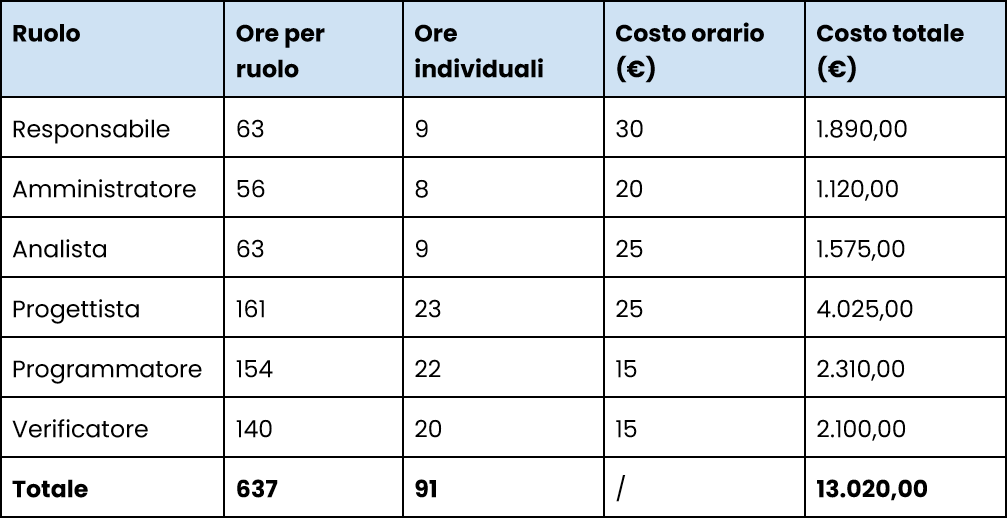
\includegraphics[width=0.75\textwidth]{assets/tabellacosti.png}
\end{figure}

\subsection{Distribuzione dei ruoli}

\subsubsection{Progettista e Programmatore}
A seguito di un'accurata valutazione delle caratteristiche richieste dalla Proponente (come ad esempio la formulazione di un dizionario dati), è stato ritenuto appropriato assegnare maggiori risorse alla fase di design e progettazione. Tale scelta è dovuta alla natura iterativa del progetto, che richiede più fasi di sperimentazione che di codifica: a questo proposito è stato ritenuto più cauto destinare al Progettista più ore che al Programmatore.\\
Tenendo conto che il costo orario del Progettista è più elevato rispetto al Programmatore, il costo totale del progetto supererà la soglia di 12.000,00 €.

\subsubsection{Responsabile di progetto}
Il responsabile di progetto si occupa di monitorare e coordinare le attività del gruppo, garantendo il rispetto delle scadenze e delle aspettative del committente sia per il software che per la documentazione. Tra le sue competenze vi è anche la comunicazione con il cliente e il committente, oltre alla gestione di eventuali conflitti. Tuttavia, si tratta della posizione più onerosa dal punto di vista economico. Di conseguenza, il team si impegna a ricoprire il ruolo nel modo più efficiente possibile, riservandogli un numero inferiore di ore rispetto al Progettista, al Programmatore e al Verificatore.

\subsubsection{Analista}
Alla figura dell'Analista è stato assegnato un impegno orario pari al Responsabile e maggiore rispetto all'Amministratore: questo perché il capitolato pone un'enfasi significativa sul machine learning, e per una buona valutazione è richiesta un'altrettanta buona comprensione del dominio applicativo.Il ruolo dell'analista è essenziale nelle fasi iniziali del progetto, specialmente durante l’analisi dei requisiti. Tuttavia, nel corso dello sviluppo, questo ruolo potrebbe richiedere una copertura minore, considerando la relativa stabilità dei requisiti del capitolato ChatSQL. Per questo motivo le ore riservate all'analista sono leggermente inferiori alla media.

\subsubsection{Amministratore}
Il gruppo ha deciso di assegnare all'amministratore un numero inferiore di ore rispetto all’Analista e al Responsabile perché, sebbene si occupi di attività significative come la gestione delle risorse a supporto del way of working, si ritiene che non debba sostenere carico di lavoro eccessivo.

\subsubsection{Verificatore}
Il verificatore svolge un ruolo fondamentale nel progetto, essendo responsabile della costante valutazione del rispetto degli standard di qualità del software e della documentazione. Il team prevede che il verificatore partecipi attivamente fino alla revisione finale, pertanto è stato assegnato un numero di ore elevato per questa figura.

\begin{figure}[H]
  \centering
  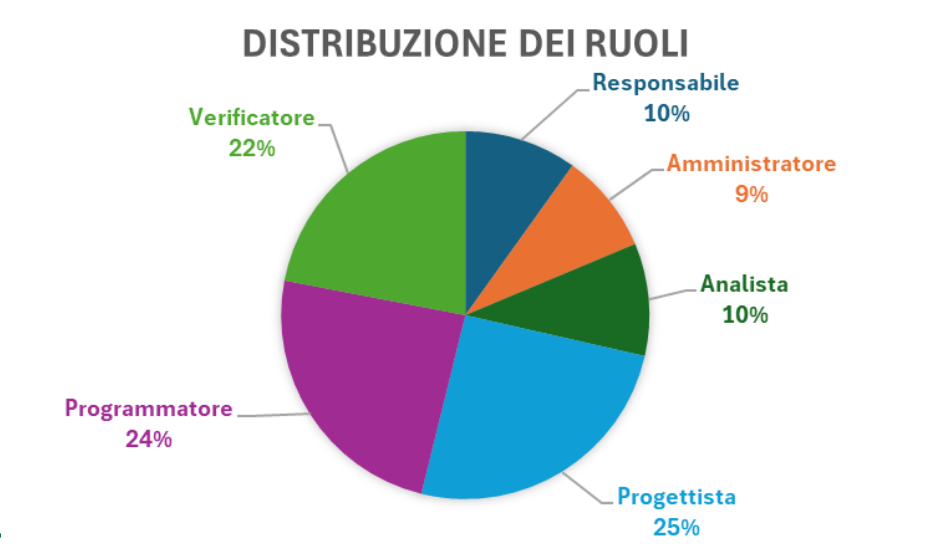
\includegraphics[width=0.75\textwidth]{assets/piechart.png}
\end{figure}

\subsection{Preventivo dei costi}
A seguito della stima delle ore totali necessarie allo svolgimento del capitolato e la suddivisione dei ruoli riportati nella tabella, si prevede un costo finale pari a \textbf{13.020,00 €}.

\section{Scadenza di consegna}
La data di scadenza ipotizzata per la consegna del prodotto finale, relativo al capitolato ChatSQL proposto da Zucchetti S.p.A., è fissata per il \textbf{13 Settembre 2024}.

\subsection{Timeline di periodi di consegna e pianificazione} \label{pianificazione}

\begin{figure}[H]
  \centering
  
\includegraphics[width=0.75\textwidth]{assets/timelineperiodi.png}
\end{figure}

\subsubsection{Kick off: 3 Aprile 2024}
Considerando l’imminente periodo festivo (riportato nella tabella dei rischi correlati a periodi di rallentamento), il kick off del progetto è fissato per il 3 aprile 2024. Avendo la scadenza stimata il 13 settembre, il tempo disponibile è di 23 settimane, suddivise in macro intervalli corrispondenti alle fasi descritte in seguito.

\subsubsection{RTB: 27 Maggio - 7 Giugno 2024}
Per la finalizzazione dell’RTB il gruppo ha preventivato un periodo di 8-10 settimane. Questo periodo è finalizzato allo sviluppo del PoC (Proof of Concept), con lo scopo di dimostrare la fattibilità dei concetti esposti nel capitolato C9. Il flusso di lavoro sarà suddiviso in sprint della durata di due settimane, alla fine dei quali verrà definito un consuntivo e organizzata una riunione per discutere il lavoro svolto e stabilire azioni di miglioramento per le iterazioni successive. Come pianificato nella sezione \ref{assunzioneimpegni}, ad ogni sprint i membri del team ruoteranno i ruoli di progetto. \\
\\
Questa macro-fase è accompagnata dall’elaborazione dei seguenti documenti di progetto:
\begin{enumerate}
  \item \textbf{Piano di progetto:} una pianificazione dettagliata che guida il team attraverso il ciclo di vita del progetto, dalle fasi iniziali alla consegna finale del prodotto software.
  \item \textbf{Piano di qualifica:} definizione di strategie e approcci per garantire il rispetto degli standard di qualità definiti e come misurarli. 
  \item \textbf{Analisi dei requisiti:} descrizione dei requisiti e dei casi d'uso del capitolato ChatSQL, rilevati dall'analisi del documento di presentazione proposto da Zucchetti S.p.A. e dalle successive riunioni con la Proponente.
  \item \textbf{Glossario:} una raccolta dei termini e dei concetti fondamentali nel contesto dell'ingegneria del software e del progetto, opportunamente catalogati per agevolare l'individuazione. Ogni voce è accuratamente corredata da una definizione specifica redatta dai membri del gruppo Argo, accompagnata da ogni altra informazione rilevante per una completa comprensione del concetto in questione.
  \item \textbf{Norme di progetto:} processi, pratiche, strumenti e norme che guidano il modo in cui il lavoro viene pianificato, eseguito, monitorato e valutato.
\end{enumerate}

\paragraph{Pianificazione RTB}
Durante il primo sprint, il gruppo si impegna a individuare e studiare, anche mediante sessioni collaborative, le tecnologie individuate dalla Proponente o dal team stesso. Inoltre, verranno programmati degli incontri con l’azienda per stabilire il way of working e le modalità di comunicazione tra cliente e fornitore, oltre a formulare una prima analisi dei requisiti e una prima definizione del PoC. Le iterazioni rimanenti saranno incentrate sullo sviluppo del PoC.

\subsubsection{PB: 13 Settembre 2024}
Per la finalizzazione della PB abbiamo preventivato un periodo di 14 settimane. Questo periodo è finalizzato allo sviluppo del MVP (Minimum Viable Product), ossia un prodotto che rispetti le caratteristiche minime evidenziate nel documento di analisi dei requisiti. \\
\\
Questa macro-fase è accompagnata dall’elaborazione dei seguenti documenti di progetto, oltre al continuo aggiornamento e miglioramento dei documenti prodotti nella fase precedente:
\begin{enumerate}
  \item \textbf{Manuale utente:} l’insieme delle informazioni utili per favorire il corretto utilizzo del prodotto software;
  \item \textbf{Specifiche tecniche:} la definizione delle funzionalità e dell’architettura, per comprenderne i limiti di impiego e di prestazioni.
\end{enumerate}

\section{Rischi e mitigazione}
Durante l’avanzamento del progetto, si prevede la possibilità di incorrere in ostacoli che, se non gestiti, potrebbero rallentare significativamente il flusso di lavoro e intaccare la pianificazione. In merito alla gestione dei rischi, è stata effettuata un’analisi preliminare per individuare quelli potenzialmente dannosi e definire delle contromisure.

\subsection{Rischi sugli strumenti software}
\begin{itemize}
  \item Probabilità: Media.
  \item Grado di criticità: Alto.
  \item Descrizione: Utilizzo di tecnologie sconosciute. Nessun membro del gruppo ha esperienza con gli strumenti e le librerie suggerite dalla Proponente; di conseguenza, l’avanzamento del progetto rischia di subire rallentamenti dovuti all’apprendimento delle nuove tecnologie.
  \item Strategie di rilevamento: Analisi, individuale e/o collaborativa, per valutare la curva di apprendimento.
  \item Contromisure: Studio preventivo o, qualora fosse necessario, sospensione del lavoro per dedicarsi all’approfondimento di una determinata tecnologia, magari attraverso sessioni collaborative volte ad allineare più rapidamente le conoscenze del gruppo.
\end{itemize}

\subsection{Rischi sugli strumenti hardware}
\begin{itemize}
  \item Probabilità: Bassa.
  \item Grado di criticità: Basso.
  \item Descrizione: Malfunzionamento degli strumenti hardware.
  \item Strategie di rilevamento: Controllo ripetuto da parte di ciascun componente del gruppo sulla propria strumentazione.
  \item Contromisure: Il lavoro viene svolto in un ambiente condiviso, al fine di limitare la perdita di informazioni.
\end{itemize}

\subsection{Rischi correlati a problemi personali}
\begin{itemize}
  \item Probabilità: Alta.
  \item Grado di criticità: Medio.
  \item Descrizione: Alcuni componenti del gruppo hanno un lavoro part-time o full-time, che potrebbe impedire loro il raggiungimento delle ore produttive richieste settimanalmente. Questo fattore, unito agli impegni personali e/o universitari, può causare difficoltà nella gestione del budget.
  \item Strategie di rilevamento: Tracciamento delle attività in un luogo comune e accessibile a tutti i membri.
  \item Contromisure: Riassegnazione delle attività e suddivisione del carico di lavoro in modo adeguato. Nel caso in cui un membro del team non sia in grado di dedicare un numero minimo di ore settimanali o di completare le attività assegnate entro la scadenza prevista, il gruppo si impegna a fornire copertura totale. Questo implica una distribuzione quanto più equa possibile delle attività tra i membri rimanenti del gruppo. Per mantenere un flusso di lavoro sostenibile, è essenziale colmare eventuali discrepanze orarie e produttive nelle settimane immediatamente successive.
\end{itemize}

\subsection{Rischi relativi a rallentamenti}
\begin{itemize}
  \item Probabilità: Alta.
  \item Grado di criticità: Basso.
  \item Descrizione: Durante il corso del progetto saranno presenti periodi di rallentamento dovuti a fattori esterni (giorni festivi, impegni studenteschi) o altri al momento non prevedibili.
  \item Strategie di rilevamento: Monitoraggio continuo delle ore dedicate dai membri del gruppo; controllo del calendario per verificare la vicinanza a date particolari (tra cui quelle indicate in tabella).
  \item Contromisure: La stima della data di consegna è stata adattata tenendo conto di questo rischio.
\end{itemize}

%% Tabella periodi
\bgroup
\begin{center}
  \begin{longtable}{|>{\centering}P{4cm}|>{\centering}P{4cm}|>{\centering\arraybackslash}P{4cm}|}
    \hline \textbf{Periodo} & \textbf{Da} & \textbf{A} \\ \hline
    \endfirsthead
    \hline \textbf{Periodo} & \textbf{Da} & \textbf{A} \\ \hline
    \endhead

    \hline \multicolumn{3}{|r|}{{Continua nella prossima pagina}} \\ \hline
    \endfoot
  
    \hline \hline
    \endlastfoot
  
    \hline Pasquale & 2024-03-29 & 2024-04-02 \\
    \hline Ponte 25 Aprile & 2024-04-25 & 2024-04-28 \\
    \hline Sessione estiva & 2024-06-17 & 2024-07-20 \\
    \hline Sessione autunnale & 2024-08-19 & Termine progetto \\
    \hline
  \end{longtable}
\end{center}
\egroup

\subsection{Rischi relativi alla collaborazione}
\begin{itemize}
  \item Probabilità: Bassa.
  \item Grado di criticità: Alto.
  \item Descrizione: Idee, metodologie e tempistiche di lavoro differenti.
  \item Strategie di rilevamento: il responsabile in carica monitora costantemente le attività e le relazioni tra i task.
  \item Contromisure: Suddivisione dei compiti, stesura e miglioramento continuo di un way of working condiviso. 
\end{itemize}

\subsection{Rischi relativi all'inesperienza}
\begin{itemize}
  \item Probabilità: Alta.
  \item Grado di criticità: Alto.
  \item Descrizione: La complessità del progetto e l’inesperienza del gruppo potrebbero portare a una sottostima del tempo o delle risorse necessarie per completare determinate attività.
  \item Strategie di rilevamento: Continuo confronto e condivisione delle conoscenze tra i membri del gruppo. In caso di valutazioni errate o difficoltà nella gestione del carico di lavoro, ciascun componente deve informare tempestivamente il resto del gruppo, così da mitigare gli impatti negativi sui task successivi.
  \item Contromisure: Riunioni interne per discutere delle problematiche e, qualora fosse necessario, suddividere le attività in sotto-attività più semplici. Inoltre, i membri del gruppo si impegnano a fornire assistenza al fine di rendere pari le competenze necessarie.
\end{itemize}

\subsection{Rischi sulla rotazione dei ruoli}
\begin{itemize}
  \item Probabilità: Alta.
  \item Grado di criticità: Alto.
  \item Descrizione: Ciascun componente del gruppo deve assumere, a turno, tutti i ruoli del progetto. Come previsto, alcuni ruoli rappresentano un’assoluta novità rispetto all’approccio comunemente adottato per la realizzazione di progetti didattici. C'è un'alta probabilità che i membri del gruppo possano trovarsi in difficoltà nello svolgere compiti inediti, soprattutto quelli di natura amministrativa e gestionale fondamentali per monitorare e garantire l'avanzamento del progetto.
  \item Strategie di rilevamento: Confronto continuo attraverso i canali di comunicazione stabiliti nel way of working.
  \item Contromisure: Organizzazione di riunioni interne all’inizio di ogni iterazione per anticipare e risolvere eventuali dubbi e ostacoli nelle attività critiche. I membri più esperti si impegnano a condividere le loro competenze con il resto del team.
\end{itemize}

\subsection{Rischi relativi al preventivo}
\begin{itemize}
  \item Probabilità: Media.
  \item Grado di criticità: Alto.
  \item Descrizione: Forte variazione tra preventivo e consuntivo, con relativo aumento dei costi.
  \item Strategie di rilevamento: Controllo periodico dello stato di avanzamento delle attività, rendicontazione delle ore.
  \item Contromisure: Preventivare le attività tenendo conto di una fase di slack.
\end{itemize}

\begin{samepage}

  \vspace*{\fill}
  Luogo e Data: \\
  Padova (PD) 2024-06-22
  \vspace*{18pt}

  \begin{tikzpicture}[overlay]
    \node [anchor = south west] at (0cm,-0.14cm) {Firma:};
    % Firma interna da sistemare
    %\node [anchor = south east] at (\textwidth- -1cm,-1.3cm) {
\includegraphics[width=8cm]{\ModelAssets{signatures/firma_sebastiano.png}}}; 
    \draw [anchor = south west] (1.5cm,0cm) -- (\columnwidth,0cm);
  \end{tikzpicture}
  
  \vspace*{20pt}
\end{samepage}


\end{document}
